\documentclass[hyperref]{article}
%MS%%%%%%%%%%%%%%%%%%%% Article Format %%%%%%%%%%%%%%%%%
%+++++++++++++++++++++ Usepackage +++++++++++++++%%
\usepackage{graphicx} %% Package for Figure
\usepackage{float} %% Package for Float
\usepackage{amssymb}
\usepackage{amsmath}
\usepackage{mathtools}
\usepackage[thmmarks,amsmath]{ntheorem} %% If amsmath is applied, then amsma is necessary
\usepackage{bm} %% Bold Mathematical Symbols
\usepackage[colorlinks,linkcolor=cyan,citecolor=cyan]{hyperref}
\usepackage{extarrows}
\usepackage[hang,flushmargin]{footmisc} %% Let the footnote not indentation
\usepackage[square,comma,sort&compress,numbers]{natbib} %% Sort of References
\usepackage{mathrsfs} %% Swash letter
\usepackage[font=footnotesize,skip=0pt,textfont=rm,labelfont=rm]{caption,subcaption} 
%% Format of Caption for Tab. and Fig.
\usepackage{booktabs} %% tables with three lines
\usepackage{tocloft}
\usepackage{graphicx}

\usepackage{algorithm}  
%\usepackage{algorithmicx}  
\usepackage{algorithmic}
%+++++++++++++++ Proof etc. +++++++++++++++++++++++++%%
{%% Environment of Proof
	\theoremstyle{nonumberplain}
	\theoremheaderfont{\bfseries}
	\theorembodyfont{\normalfont}
	\theoremsymbol{\mbox{$\Box$}}
	\newtheorem{proof}{Proof}
}

\usepackage{theorem}
\newtheorem{theorem}{Theorem}[section]
\newtheorem{lemma}{Lemma}[section]
\newtheorem{definition}{Definition}[section]
\newtheorem{assumption}{Assumption}[section]
\newtheorem{example}{Example}[section]
\newtheorem{corollary}{Corollary}[section]
{%% Environment of Remark
	\theoremheaderfont{\bfseries}
	\theorembodyfont{\normalfont}
	\newtheorem{remark}{Remark}[section]
}
\usepackage{abstract}
\renewcommand{\abstractnamefont}{\Large\bfseries}
%\numberwithin{equation}{section} %% Number of Equation
%++++++++++++++++++++++++++++++++ Page format ++++++++++++++++++++++++++%%
\graphicspath{{figure/}}                                 %% Path of Figures
\usepackage[a4paper]{geometry}                           %% Paper size
\geometry{left=2.5cm,right=2.5cm,top=2.5cm,bottom=2.5cm} %% Margin
\linespread{1.2}      

% matlab code package
\usepackage{appendix}
\usepackage{listings}%插入代码
\usepackage{color}
\lstset{%代码格式的配置
	extendedchars=false,            % Shutdown no-ASCII compatible
	language=Matlab,                % !!!选择代码的语言
	basicstyle=\footnotesize\tt,    % the size of the fonts that are used for the code
	tabsize=3,                            % sets default tabsize to 3 spaces
	numbers=left,                   % where to put the line-numbers
	numberstyle=\tiny,              % the size of the fonts that are used for the line-numbers
	stepnumber=1,                   % the step between two line-numbers. If it's 1 each line
	% will be numbered
	numbersep=5pt,                  % how far the line-numbers are from the code   %
	keywordstyle=\color[rgb]{0,0,1},                % keywords
	commentstyle=\color[rgb]{0.133,0.545,0.133},    % comments
	stringstyle=\color[rgb]{0.627,0.126,0.941},      % strings
	backgroundcolor=\color{white}, % choose the background color. You must add \usepackage{color}
	showspaces=false,               % show spaces adding particular underscores
	showstringspaces=false,         % underline spaces within strings
	showtabs=false,                 % show tabs within strings adding particular underscores
	frame=single,                   % adds a frame around the code
	captionpos=b,                   % sets the caption-position to bottom
	breaklines=true,                % sets automatic line breaking
	breakatwhitespace=false,        % sets if automatic breaks should only happen at whitespace
	title=\lstname,                 % show the filename of files included with \lstinputlisting;
	% also try caption instead of title
	mathescape=true,escapechar=?    % escape to latex with ?..?
	escapeinside={\%*}{*)},         % if you want to add a comment within your code
	%columns=fixed,                  % nice spacing
	%morestring=[m]',                % strings
	%morekeywords={%,...},%          % if you want to add more keywords to the set
	%    break,case,catch,continue,elseif,else,end,for,function,global,%
	%    if,otherwise,persistent,return,switch,try,while,...},%
}
%\usepackage{enumitem}
% \setlength{\parskip}{0.4em}

                                   %% Line Spread
%MS%%%%%%%%%%%%%%%%%%%%%%%%%%%% End Format %%%%%%%%%%%%%%%%%%%%%%%%%%%%%%%%%%

%MS%%%%%%%%%%%%%%%%%%%%%%%%%%%%%%%%%%%%%%%%%%%
%MS                                         %%
%MS        The Main Body begins here        %%
%MS                                         %%
%MS%%%%%%%%%%%%%%%%%%%%%%%%%%%%%%%%%%%%%%%%%%%

%MS++++++++++++++++++++++++++++++ Title +++++++++++++++++++
\title{ME5413 Autonomous Mobile Robotics: \\ Homework 2}
\author{\textup{Chen Yihui \ \ \ A0263115N \\ Wang Renjie \ A0263387U }}
\begin{document}
	\begin{titlepage}
		\center
		\newcommand{\HRule}{\rule{\linewidth}{0.5mm}}
		
\includegraphics[width=8cm]{logo.png}\\[1cm] 
		\quad\\[2cm]
		\textsl{\Large National University of Singapore}\\[0.5cm] 
		\textsl{\large College of Design and Engineering}\\[0.5cm]
		\makeatletter
		\HRule \\[0.4cm]
		{ \huge \bfseries \@title}\\[0.4cm] 
		\HRule \\[2cm]
		\begin{minipage}{0.4\textwidth}
			\begin{flushleft} \large
				\emph{Group 9:}\\
				\@author 
			\end{flushleft}
		\end{minipage}
		~
		\begin{minipage}{0.4\textwidth}
			\begin{flushright} \large
				\emph{Supervisor:} \\
				\textup{Prof. Marcelo H Ang Jr}
			\end{flushright}
		\end{minipage}\\[3cm]
		\makeatother
		%{\large \emph{Matriculation Number: A0263115N}}\\[0.5cm]
		{\large \emph{Email Address: e1010473@u.nus.edu \\	\ \ \ \ \ \ \ \ \ \ \ \ \ \ \ \ \ \ \ \ e1010745@u.nus.edu}}\\[0.5cm]
		{\large \today}\\[2cm] 
		\vfill 
	\end{titlepage}

\section{Task 1: ICP Algorithm for Matched Point Cloud}

\hspace{1.0em}

In Task 1, we assume the correspondence is known for the two point clouds and perform ICP algorithm to do point cloud registration. Firstly, the SVD-based ICP algorithm is reviewed. 

Given the source point cloud $X=\{x_{1}, x_{2}, ..., x_{m}\}$ and target point cloud $Y=\{y_{1}, y_{2}, ..., y_{m}\}$, the task for point cloud registration is to find a rotation matrix $R$ and a translation matrix $t$ that can transform $X$ to $Y$. In other words, we need to find $R$ and $t$ to minimize the sum of the squared distance between the corresponding points in the two point clouds:

\begin{equation}
\begin{aligned}
E(R,t)&=\frac{1}{m}\sum_{i=1}^{m}\left \| y_{i}-Rx_{i}-t \right \|^{2}\\
&=\frac{1}{m}\sum_{i=1}^{m}(\left \| y_{i}-u_{y}-R(x_{i}-u_{x})\right \|^{2}+\left \| u_{y}-Ru_{x}-t\right \|^{2})
\label{eq1}
\end{aligned}
\end{equation}

where $u_{x}$ and $u_{y}$ are the centroid of the point set $X$ and $Y$, $u_{x}=\frac{1}{m}\sum_{i=1}^{m}x_{i}$ and $u_{y}=\frac{1}{m}\sum_{i=1}^{m}y_{i}$. To simplify the problem, we divide Eq.~\ref{eq1} to:

\begin{equation}
\begin{aligned}
E_{1}(R,t)=\frac{1}{m}\sum_{i=1}^{m}\left \| y_{i}-u_{y}-R(x_{i}-u_{x})\right \|^{2}, \ \ \
E_{2}(R,t)=\left \| u_{y}-Ru_{x}-t  \right \|^{2}
\label{eq2}
\end{aligned}
\end{equation}

Therefore, we can first find the $R$ to minimize $E_{1}(R,t)$ and then calculate $t$ from $E_{2}(R,t)$. Suppose $x_{i}^{'}=x_{i}-u_{x}$, $y_{i}^{'}=y_{i}-u_{y}$, the problem turns to:

\begin{equation}
\begin{aligned}
min\{E_{1}(R,t)\}=min\{\frac{1}{m}\sum_{i=1}^{m}(y_{i}^{'T}y_{i}^{'}+x_{i}^{'T}R^{T}Rx_{i}^{'}-2y_{i}^{'T}Rx_{i}^{'})\} = max \{\sum_{i=1}^{m}y_{i}^{'T}Rx_{i}^{'}\}
\label{eq3}
\end{aligned}
\end{equation}

Using the properties of trace, we derive:

\begin{equation}
\begin{aligned}
\sum_{i=1}^{m}y_{i}^{'T}Rx_{i}^{'}=\sum_{i=1}^{m}Trace(y_{i}^{'T}Rx_{i}^{'})=Trace(\sum_{i=1}^{m}Rx_{i}^{'}y_{i}^{'T})=Trace(RH)
\label{eq4}
\end{aligned}
\end{equation}

where $H=\sum_{i=1}^{m}x_{i}^{'}y_{i}^{'T}$. According to Schwarz inequality, we can maximum Eq.~\ref{eq4} by finding a $R$ that can convert $RH$ to the form of $AA^{T}$. Therefore, we apply Singular Value Decomposition (SVD) on $H$ and get $H=U\Sigma V^{T}$. Then we choose the rotation matrix:

\begin{equation}
\begin{aligned}
R=VU^{T} 
\label{eq5}
\end{aligned}
\end{equation}

Then, $RH=VU^{T}U\Sigma V^{T}=V\Sigma V^{T}=V\Sigma^{1/2}(V\Sigma^{1/2})^{T}$, which is in the form of $AA^{T}$ and we finally minimize $E_{1}(R,t)$. After obtaining $R$, we can solve the translation matrix $t$ to minimize $E_{2}(R,t)$:

\begin{equation}
\begin{aligned}
t=u_{y}-Ru_{x} 
\label{eq6}
\end{aligned}
\end{equation}

Since we have known the corresponding point pairs between source point cloud $X$ and target $Y$, we can easily get the homogeneous transformation matrix $T\in SE(3)$ by combing the rotation matrix $R\in SO(3)$ and translation matrix $t \in \mathbb{R}^{3}$ computed in Eq.~\ref{eq5} and \ref{eq6}:

\begin{equation}
\begin{aligned}
T=\begin{pmatrix}
R &t \\ 
0^{T} &1 
\end{pmatrix}
\label{eq7}
\end{aligned}
\end{equation}

The core code of ICP algorithm with comment is shown in Fig.~\ref{fig1a} and derived transformation matrix $T$ is recorded in Fig.~\ref{fig1b}. As is shown in Fig.~\ref{fig1c}, the source point cloud (red) is transformed to the blue one, which is overlapped with the target point cloud (green). The final mean error between the blue and green point clouds is about 0.226. 


\begin{figure}[H]
	\centering
	\begin{minipage}[t]{0.32\textwidth}
		\centering
		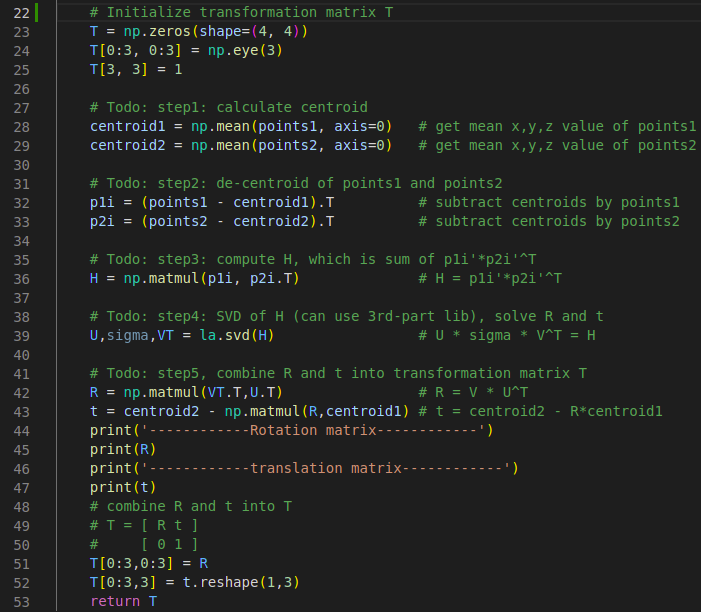
\includegraphics[width=4cm]{1_code.png}
		\subcaption{Core code for ICP algorithm}
		\label{fig1a}
	\end{minipage}
	\begin{minipage}[t]{0.32\textwidth}
		\centering
		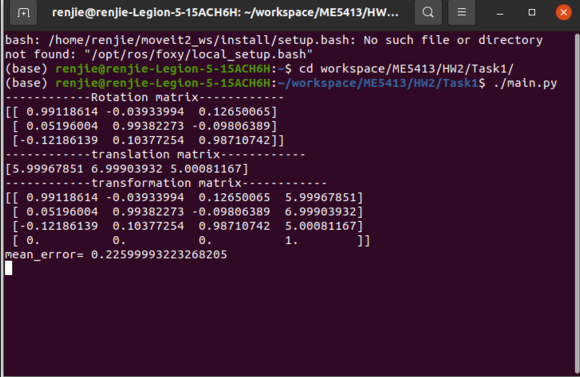
\includegraphics[width=5cm]{1_T.png}
		\subcaption{Derived transformation matrix $T$}
		\label{fig1b}
	\end{minipage}
	\begin{minipage}[t]{0.32\textwidth}
		\centering
		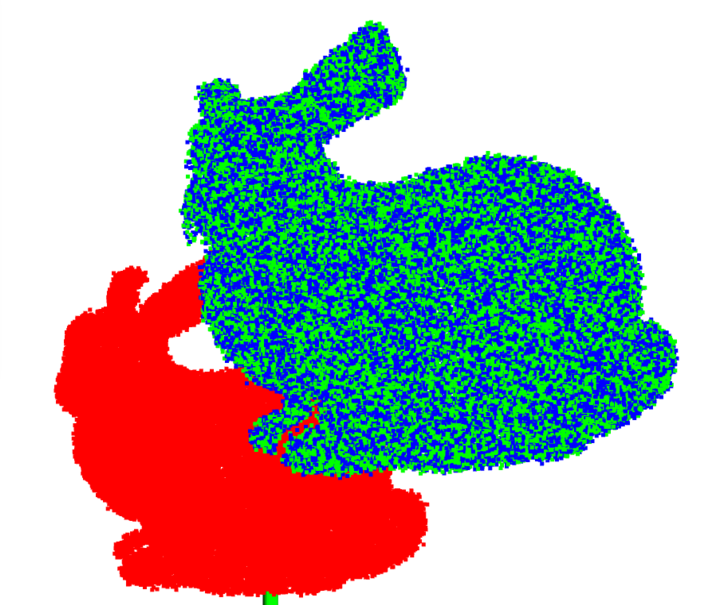
\includegraphics[width=5cm]{1_result.png}
		\subcaption{Visualization result}
		\label{fig1c}
	\end{minipage}
	\caption{Implementation of ICP algorithm for matched point cloud}
	\label{fig1}
\end{figure} 


\section{Task 2: ICP Algorithm for Unmatched Point Cloud}

\hspace{1.0em}

In real cases, the correspondence between the source and target point cloud is usually unknown. A common method is to regard the nearest neighbor point as corresponding point and solve the problem iteratively. The ICP algorithm for unmatched point cloud is given in Alg.~\ref{alg:algorithm1}.

\begin{algorithm}
	\caption{SVD-based ICP algorithm for unmatched point cloud}
	\begin{algorithmic}  
		\STATE Initialize the accumulated transformation matrix $T\_accumulated$.
		\WHILE {$error > threshold$}
		
		\STATE Step 1: Find the corresponding points from two point clouds.
		
		\STATE Step 2: Compute the transformation matrix $T$ following the steps in Task 1.
		
		\STATE Step 3: Update accmulated matrix. \ ($T\_accumulated=T*T\_accumulated$)
		
		\STATE Step 4: Apply alignment. \ ($x_{i}^{'}=T*x_{i}$)
		
		\STATE Step 5: Update error.
		
		\ENDWHILE
		
	\end{algorithmic}
	\label{alg:algorithm1} 
\end{algorithm}

The $threshold$ is set to be 0.1 and core code for the iterative ICP algorithm is shown in Fig.~\ref{fig2}. To show the more and more overlapped rabits, we record the transformation matrix $T$ and $T\_accumulated$ in iteration 7, 15 and 23, as well as visualizing the two point clouds and mean error between them (Fig.~\ref{fig3}). 

\begin{figure}[H]
	\centering
		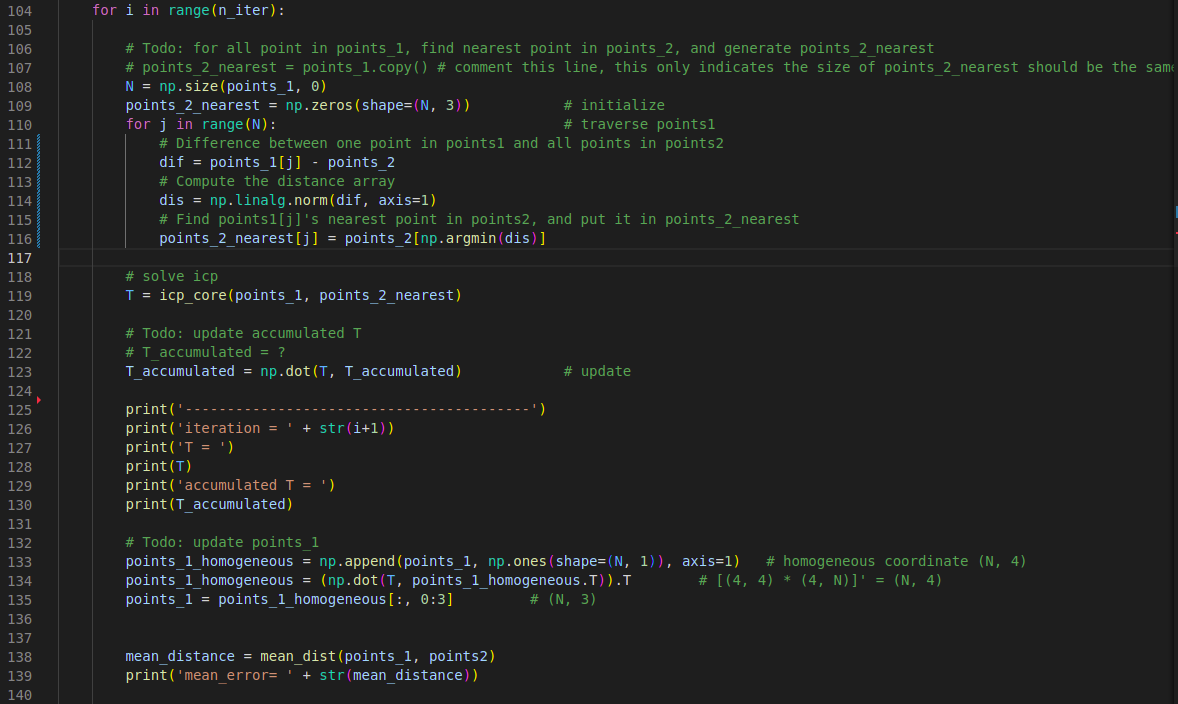
\includegraphics[width=6cm]{2_code.png}
	\caption{Code for ICP algorithm with unmatched point cloud}
	\label{fig2}
\end{figure} 

\begin{figure}[H]
	\centering
	\begin{minipage}[t]{0.32\textwidth}
		\centering
		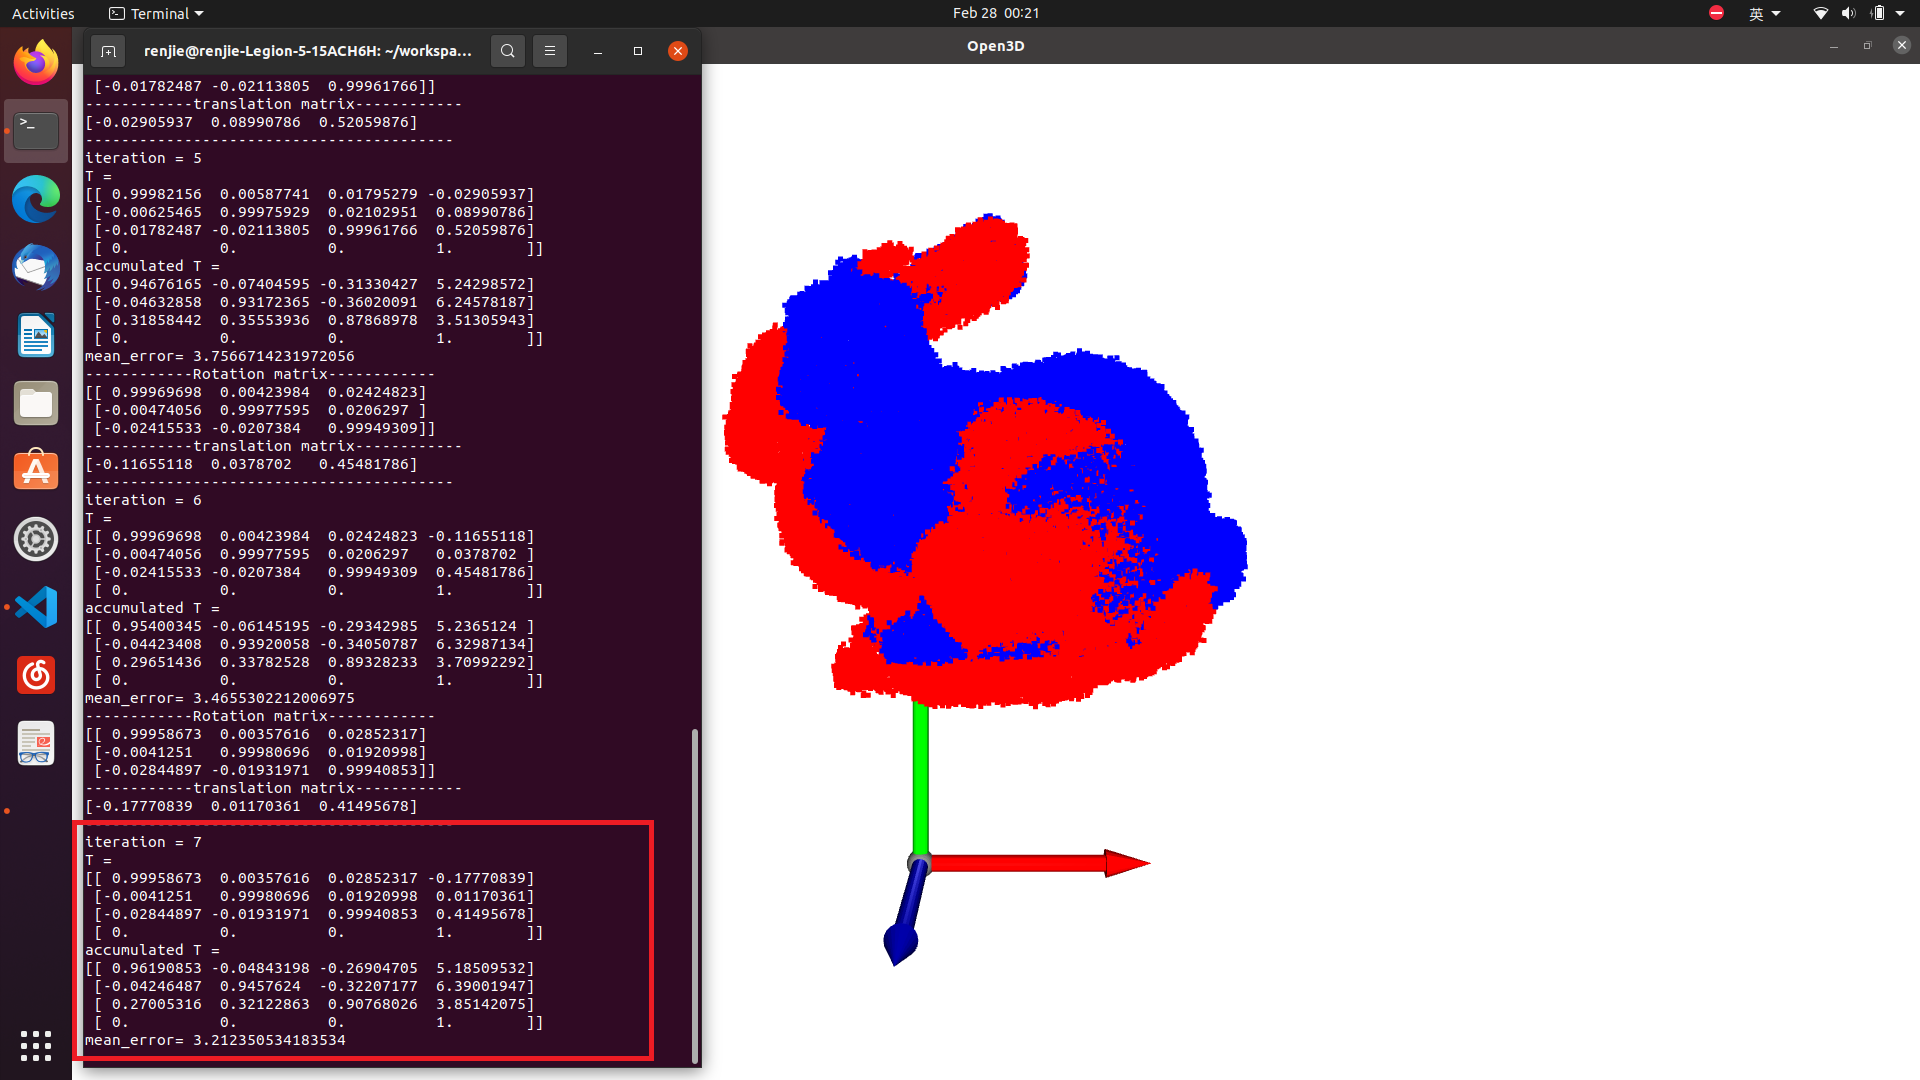
\includegraphics[width=5cm]{2_M1.png}
		\subcaption{Results at iteration 7}
		\label{fig3a}
	\end{minipage}
	\begin{minipage}[t]{0.32\textwidth}
		\centering
		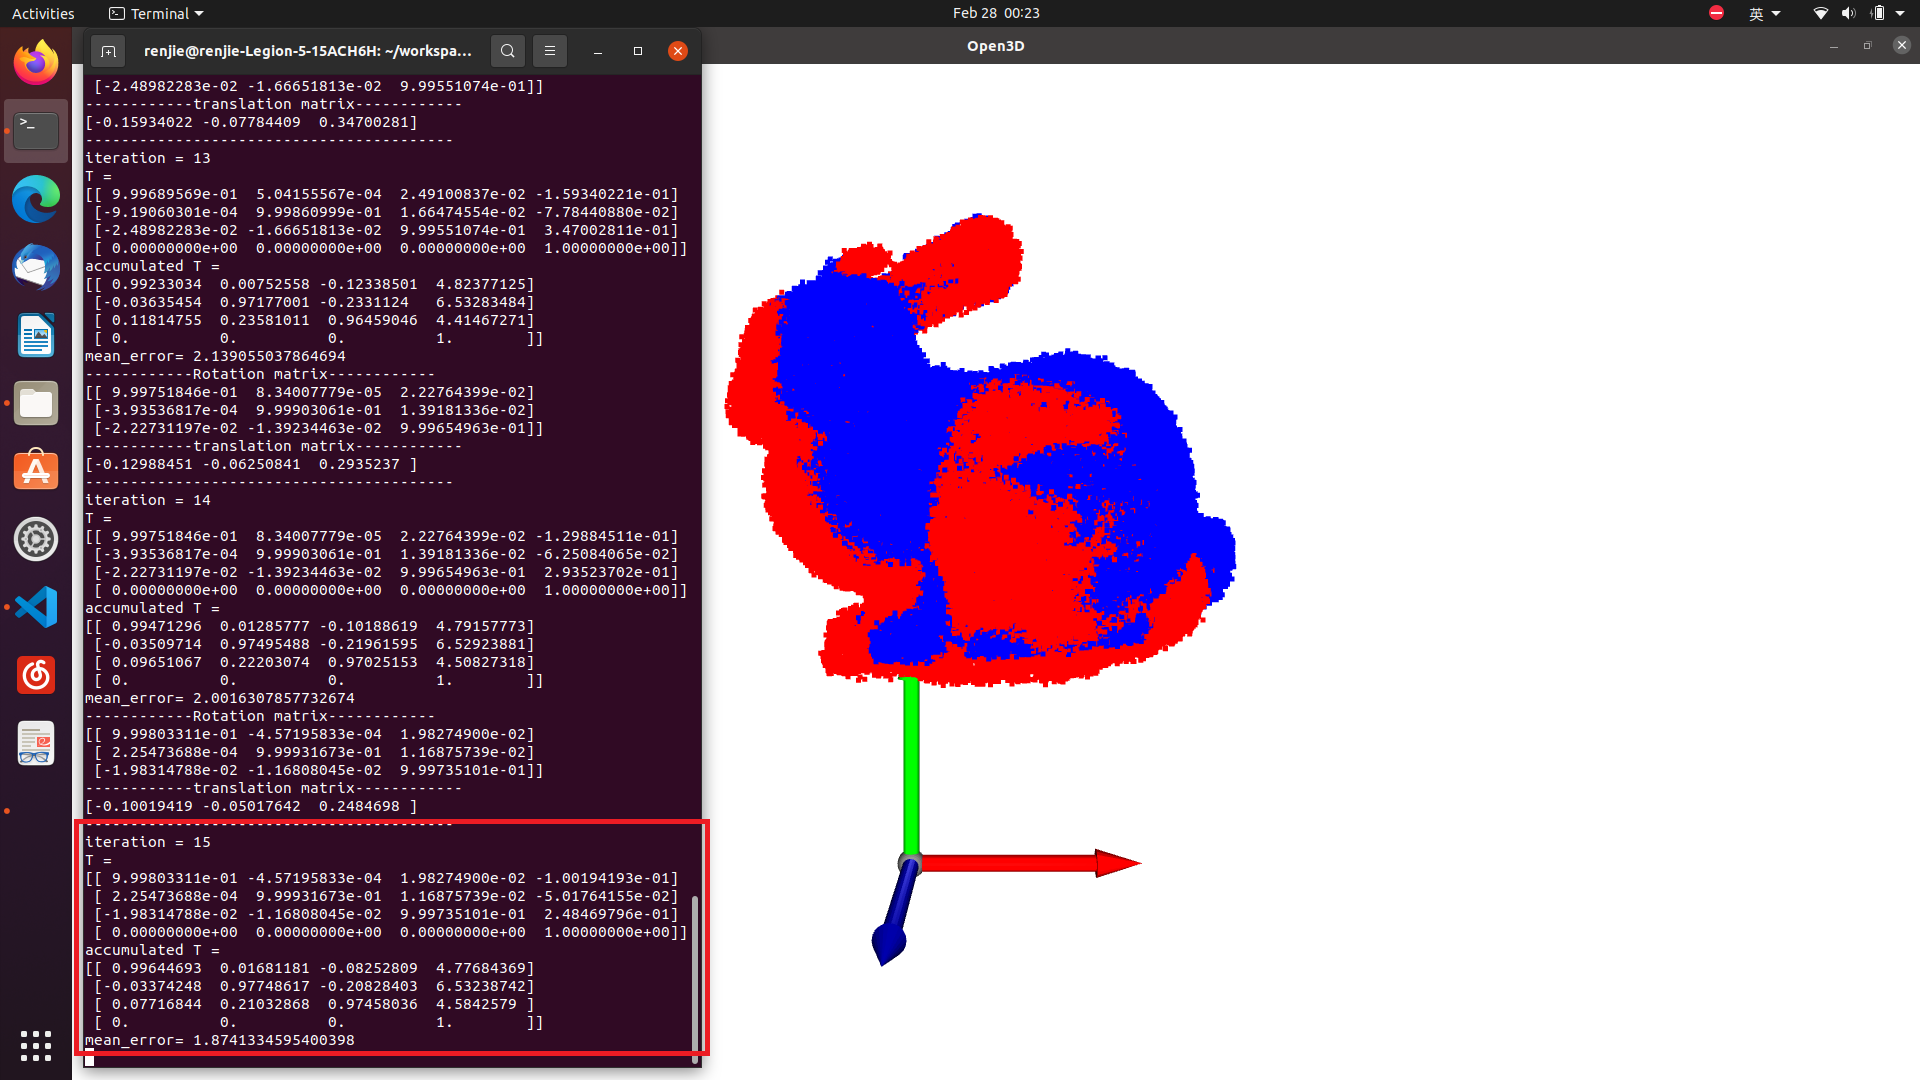
\includegraphics[width=5cm]{2_M2.png}
		\subcaption{Results at iteration 15}
		\label{fig3b}
	\end{minipage}
	\begin{minipage}[t]{0.32\textwidth}
		\centering
		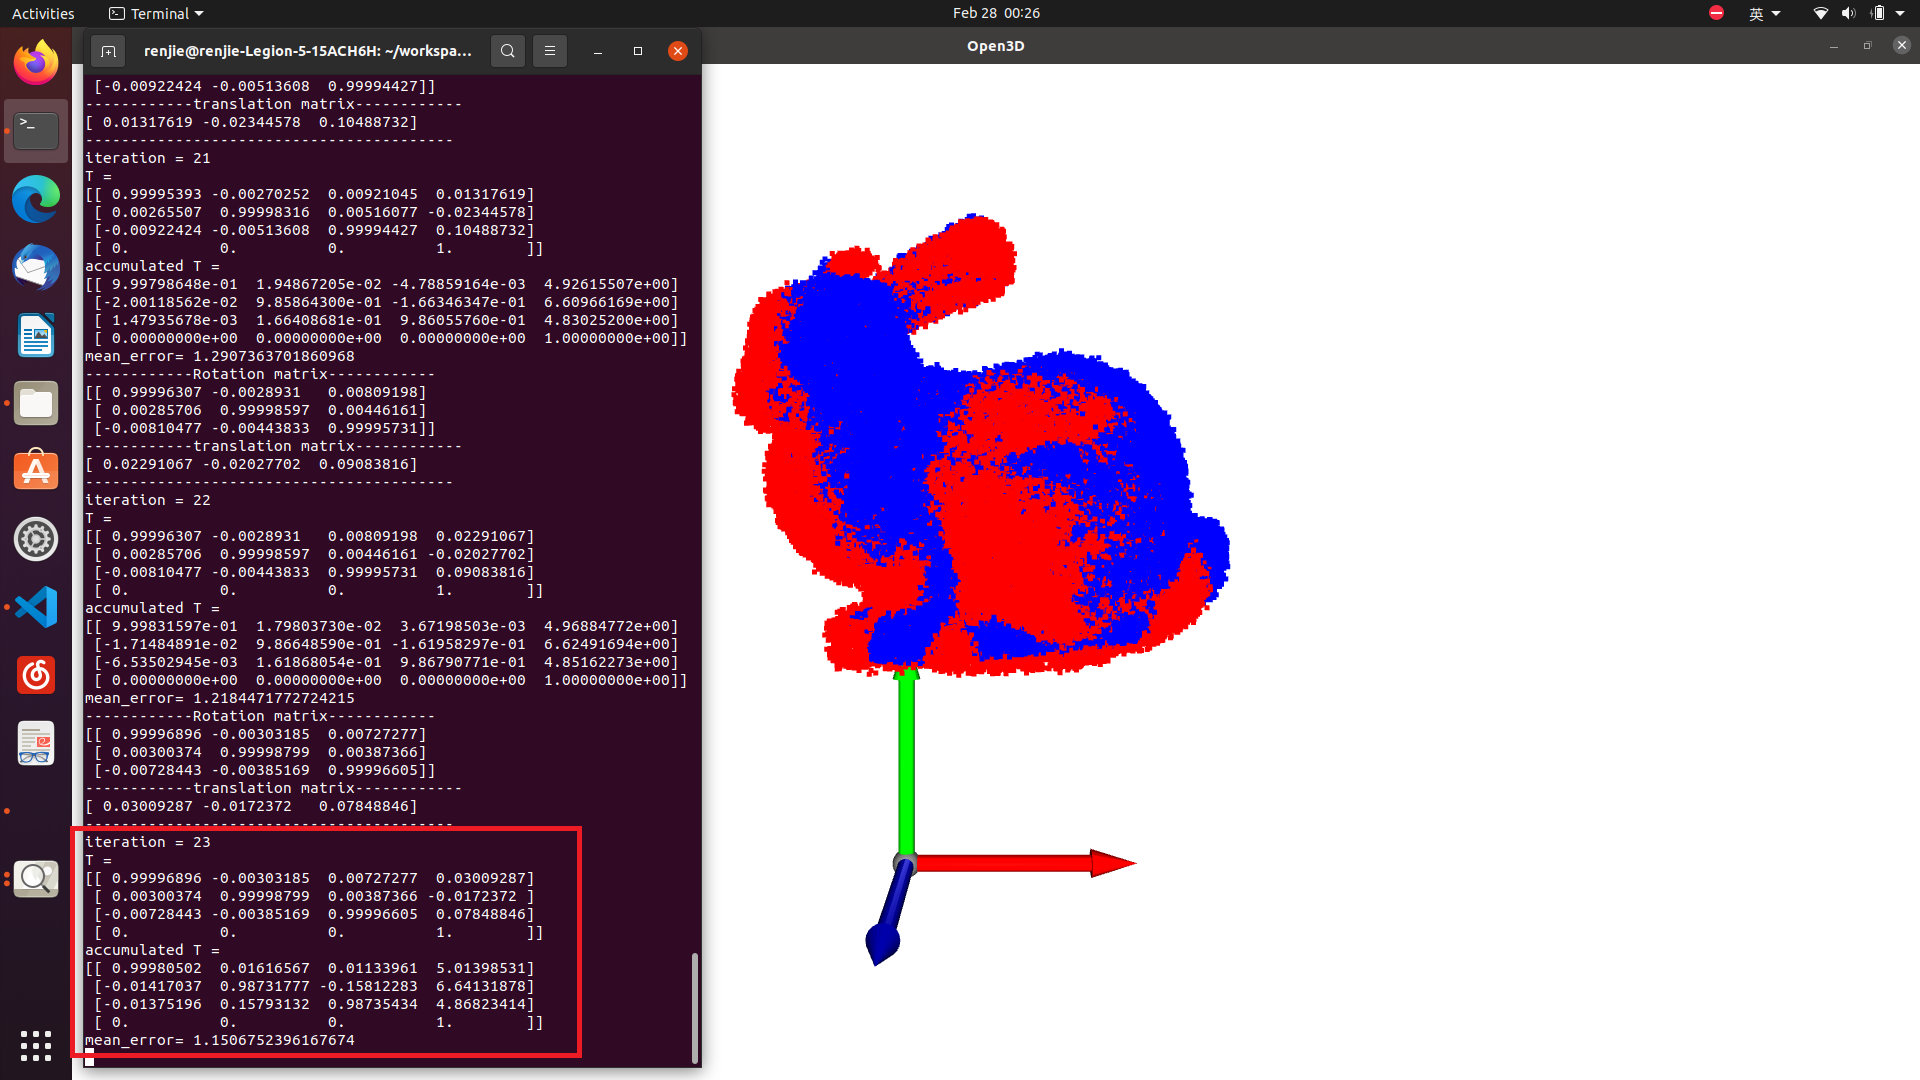
\includegraphics[width=5cm]{2_M3.png}
		\subcaption{Results at iteration 23}
		\label{fig3c}
	\end{minipage}
	\caption{Implementation of ICP algorithm for unmatched point cloud}
	\label{fig3}
\end{figure} 

We can see the mean error is reduced after each iteration (3.212 to 1.874 to 1.151), and it declines more and more slowly as iteration number increases. The final result at 30th iteration is shown in Fig.~\ref{fig4}, where the mean error is about 0.797 and still higher than the mannually set threshold. We increase the maximum iteration number to 50 and the result is shown in Fig.~\ref{fig4b}. The mean error is only ? now and the accumulated transformation matrix $T\_accumulated$ is very close to that we derived in Task1. However, the cost time is rather high (650s) because of the time-consuming corresponding points search procedure. In practice, kd-tree can be used to search for the nearest points more efficiently. Moreover, some learning-based methods have been popular for solving the point cloud registration problem. 

\begin{figure}[H]
	\centering
	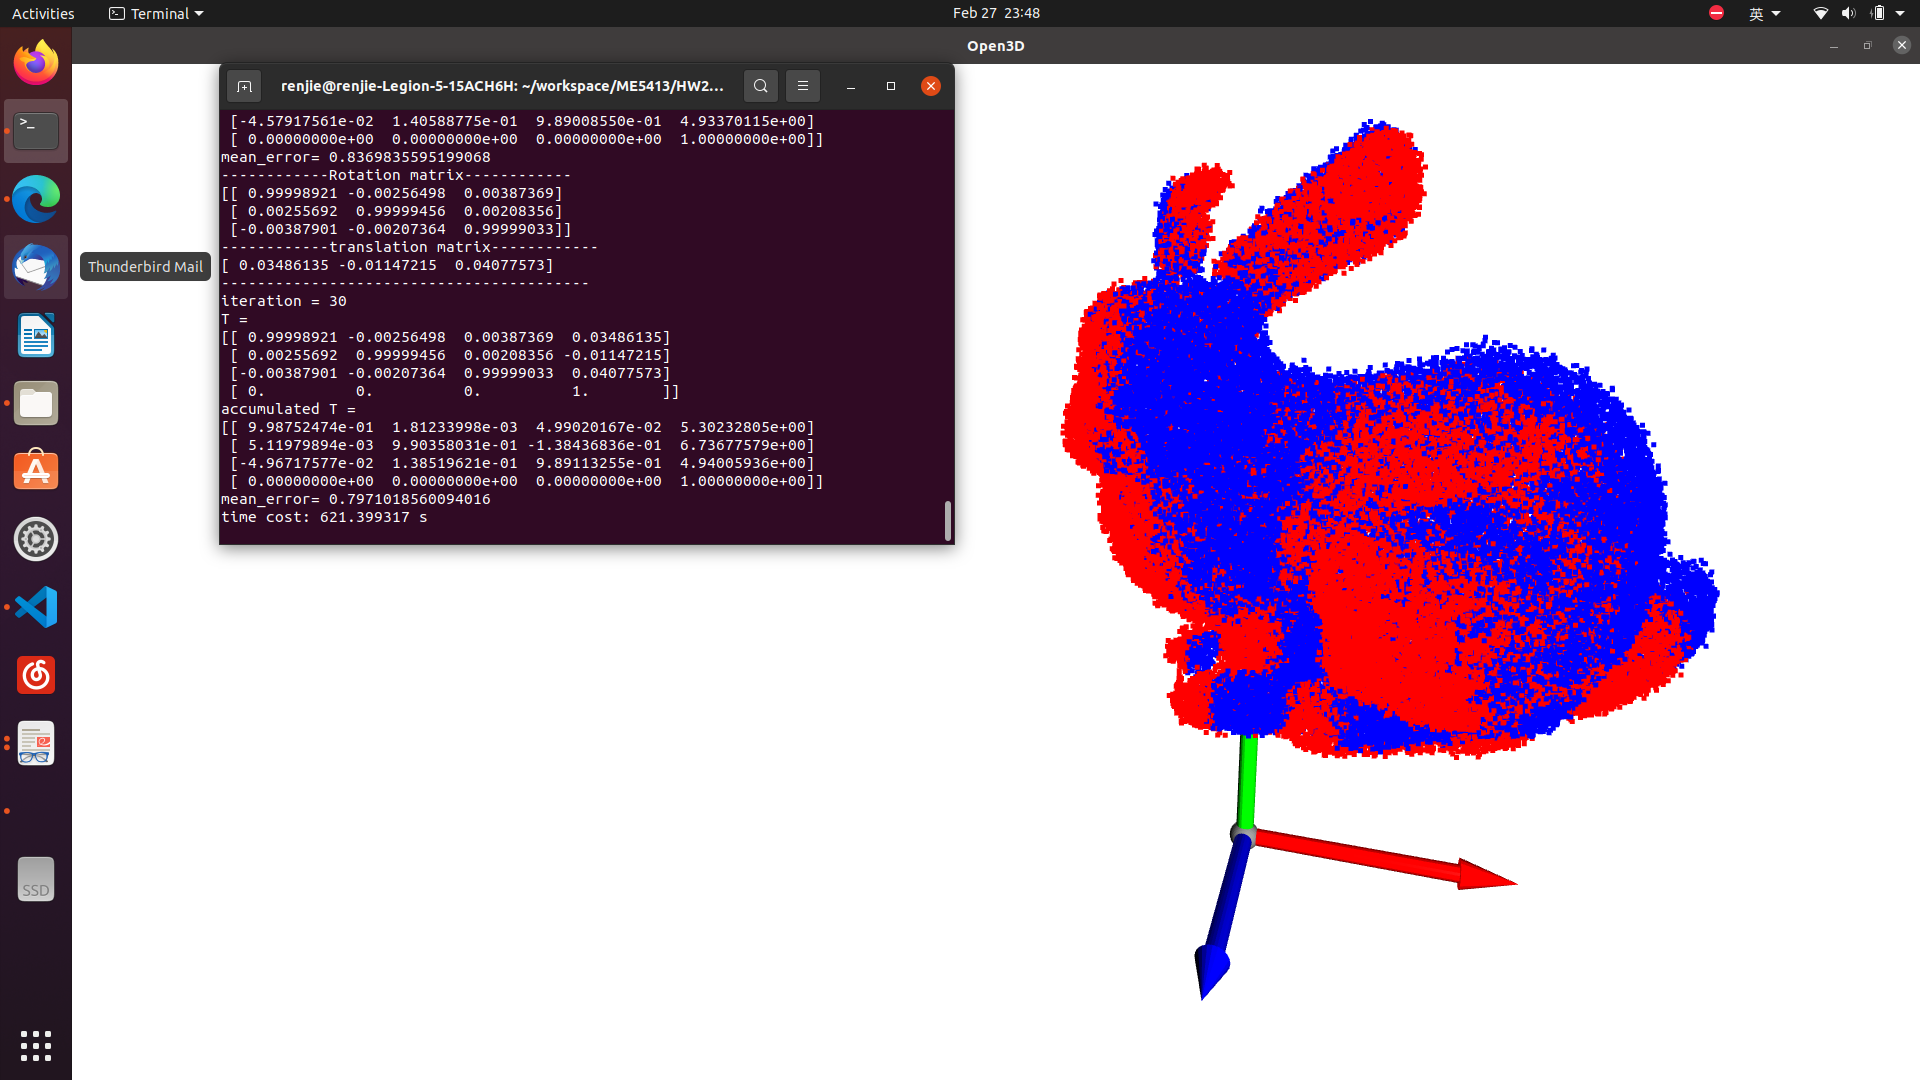
\includegraphics[width=10cm]{2.3.png}
	\caption{Code for ICP algorithm with unmatched point cloud}
	\label{fig4}
\end{figure}






\section{Task 3: Running SLAM Algorithms}

\subsection{Cartographer with 2D LiDAR}

\hspace{1.0em}


\begin{figure}[H]
	\centering
	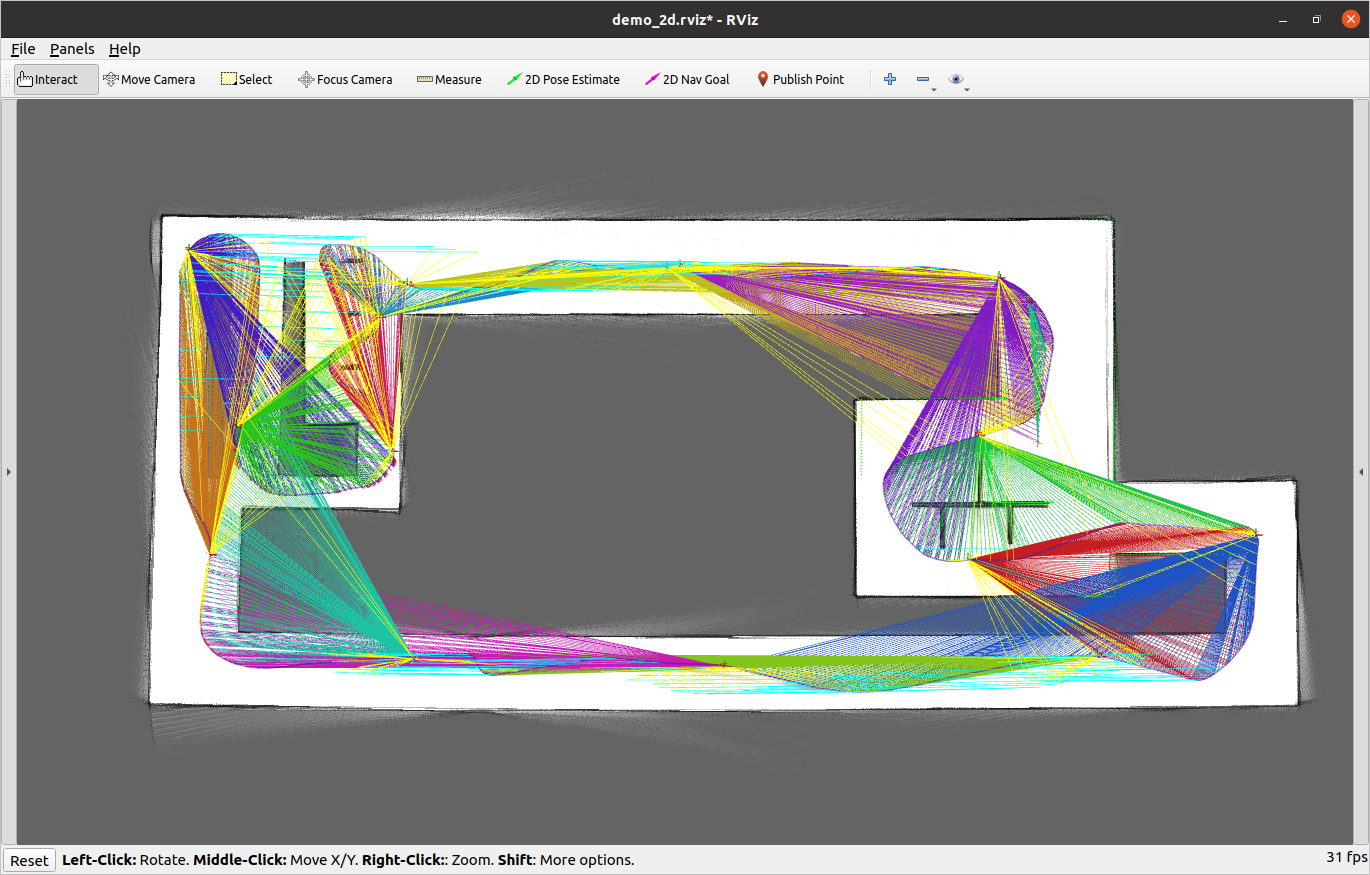
\includegraphics[width=10cm]{task3a_result.png}
	\caption{Code for ICP algorithm with unmatched point cloud}
	\label{fig5}
\end{figure}


\begin{figure}[H]
	\centering
	\begin{minipage}[t]{0.32\textwidth}
		\centering
		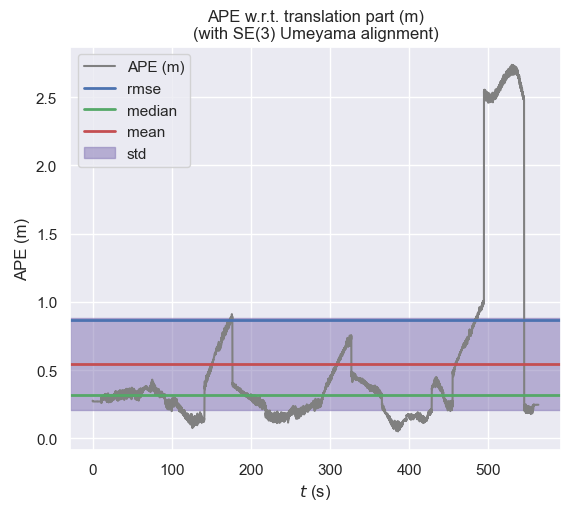
\includegraphics[width=5cm]{3a_evo1.png}
		\subcaption{Results at iteration 7}
		\label{fig6a}
	\end{minipage}
	\begin{minipage}[t]{0.32\textwidth}
		\centering
		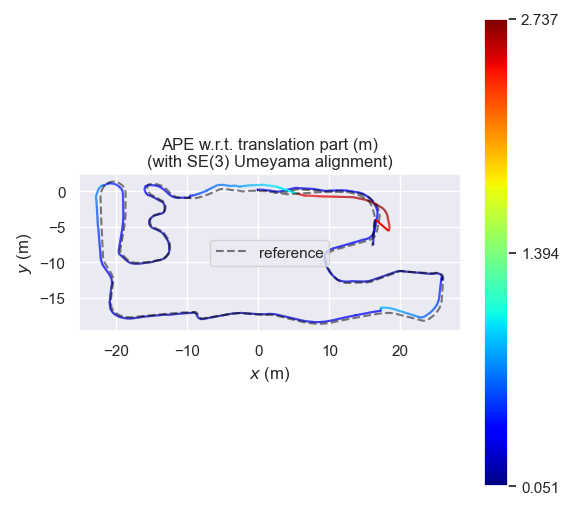
\includegraphics[width=5cm]{3a_evo2.png}
		\subcaption{Results at iteration 15}
		\label{fig6b}
	\end{minipage}
	\begin{minipage}[t]{0.32\textwidth}
		\centering
		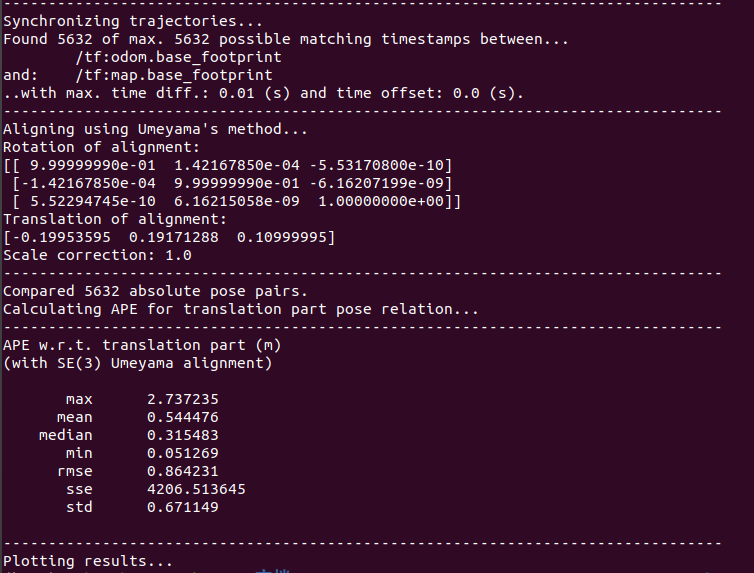
\includegraphics[width=5cm]{3a_evo3.png}
		\subcaption{Results at iteration 23}
		\label{fig6c}
	\end{minipage}
	\caption{Implementation of ICP algorithm for unmatched point cloud}
	\label{fig3}
\end{figure} 

In your report: 

•  Briefly describe the SLAM1 algorithm you choose to use 

•  Describe the detailed process of running the SLAM algorithms, give a screenshot of your 
algorithm running in rviz 

•  Highlight your modification/tuning done on the algorithms to achieve better results 

•  Show the Absolute RMSE, as well as the plots generated by the EVO tool 

•  Discuss the drawbacks/failures in your tests, provide some analysis and propose possible 
solutions (illustrate with figures and provide your hypostasis)








	
\end{document}








